\documentclass{beamer}

\usepackage{wrapfig}
\usepackage{algpseudocode}
\usepackage{algorithm}
\usepackage[export]{adjustbox}
\usepackage{svg}

\usetheme{Boadilla}
\usecolortheme{dolphin}
\setbeamertemplate{navigation symbols}{}
\setbeamertemplate{sections/subsections in toc}[sections numbered]

\setbeameroption{hide notes}
% \setbeameroption{show only notes}
% \setbeameroption{show notes on second screen=right}

\title[A Review on Debugging And Tracing]
{A Review of Debugging and Tracing Features in Hardware}
\author[]{Hossein Afkar}
\institute{DRTS Lab}
\date{\today}

\begin{document}

\frame{\titlepage}

\begin{frame}
    \frametitle{Outline}
    \tableofcontents[hideallsubsections]
\end{frame}

\AtBeginSection[]
{
    \begin{frame}{Outline}
        \tableofcontents[currentsection]
    \end{frame}
}


\section{Introduction}
\subsection{Preface}
\begin{frame}
    \frametitle{Preface}
    \note[item]{The growing complexity of embedded system hardware and software makes their
    behavior analysis a challenging task.}
    \note[item]{Having Access to facilities that
    enable us to peek deeper inside the embbeded systems is a must have
    feature.}
    \note[item]{In this review we try to investigate the tracing and debugging
    capabilities of the hardware and gain a better understanding of theirA
    features.}

    Embedded systems challenges:
    \begin{itemize}
        \item Complexity:
            \begin{itemize}
                \item Software.
                \item Hardware.
            \end{itemize}
        \item How to Peek Inside?
    \end{itemize}
    What we need:
    \begin{itemize}
        \item Tracing.
        \item Debugging.
    \end{itemize}
\end{frame}

\subsection{Definitions}
\begin{frame}
    \frametitle{Definition of Tracing}
    \note[item]{Brendan Gregg worked on the USENIX LISA Steering Committee and
    now is co-chair for Large Installation Systems Administration (LISA).}
    \note[item]{extracted from ARM's paper on understanding trace.}
    \note[item]{Operating: mode of the core. User mode kernel mode and so on and also the state of the core like sleep mode, debug mode}
    \note[item]{Execution: Process of executing instructions}
    \note[item]{Performing: The ability to execute the task in a specified
    time frame or with a certain level of efficiency}
    \note[item]{Arm Architecture Reference Manual}
    \begin{itemize}
        \item ARM: Trace refers to the process of \underline{capturing data}
            that illustrates how the components in a design are
            \underline{operating},
            \underline{executing},
            and \underline{performing}.
        \item Intel: Tracing is
            \underline{event-based} recording, where event data is captured and
            \underline{saved for later} analysis or
            \underline{consumed on-the-fly} for custom summaries and
            other actions.
    \end{itemize}
\end{frame}

\begin{frame}
    \frametitle{Definition of Debugging}
    \note[item]{Debug provides the ability to observe and control the CPU and
    system environment while executing software on a deeply embedded processor.
    The ability to debug helps to fix bugs in the software and to optimize the
    software for performance. The debug logic that is an integrated part of
    the Arm cores helps to achieve these goals}
    \note[item]{learn the architecture ARM}
    \begin{itemize}
        \item ARM: \underline{Observe} and \underline{control} the CPU and
            system environment while executing software. \\
            Goals:
            \begin{itemize}
                \item Fix bugs.
                \item Optimize software for performance.
            \end{itemize}
    \end{itemize}
\end{frame}

\subsection{Usage}
\begin{frame}
    \frametitle{Tracing and Debugging Usage}
    \note[item]{Instruction trace shows the core execution history and places where execution might behave unexpectedly.}
    \note[item]{Data trace shows what memory address was accessed and if accesses completed successfully.}
    \note[item]{Monitor the system as a whole. monitor outside signals and functionality}
    \begin{itemize}
        \item Diagnose problem during runtime:
            \begin{itemize}
                \item Unexpected behaviour.
                \item Bad memory accesses.
            \end{itemize}
        \item Measure performance:
            \begin{itemize}
                \item Cycle Count.
                \item Event timestamping.
                \item Data Accesses.
            \end{itemize}
        \item View operation on a system level.
        \item Control debugging logic:
            \begin{itemize}
                \item Breakpoints.
                \item Processor state.
            \end{itemize}
    \end{itemize}
\end{frame}

\section{JTAG: Test Access Port And Boundary Scan Architecture}
\subsection{IEEE Std 1149.1-2001}
\begin{frame}
    \frametitle{Test Access Port and Boundary Scan Architecture}
    \note[item]{1999}
    \note[item]{Since the mid-1970s testing PCBs has relied heavily on a
    technique called bed of nails.}
    \note[item]{With the growth of SMD components and the decreasing
    distance of the contact pins on the integrated circuits  a group of
    concerned test engineers in a number of European electronics systems
    companies got together to examine the problem and its possible solution.}
    PCB and IC Testing:
    \begin{itemize}
        \item Challenges:
            \begin{itemize}
                \item Increased pin count.
                \item SMD components.
                \item Physical access.
                \item Cost.
                \item No standard testing port.
            \end{itemize}
    \end{itemize}
    \begin{figure}
        \centering
        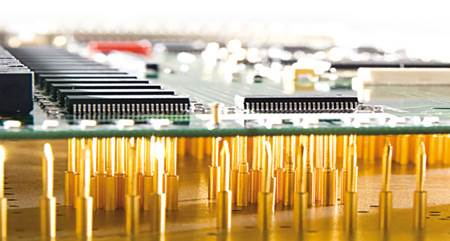
\includegraphics[width=0.50\columnwidth]{bedofnails.jpg}
        \caption{An example of a bed of nails tester}
        \label{fig:bedofnails}
    \end{figure}
\end{frame}

\begin{frame}
    \frametitle{IEEE Std 1149.1-2001}
    \note[item]{IEEE Standard Test Access Port and Boundary-Scan Architecture}
    \note[item]{Before this standard testing was heavily dependant on the bed on nails}
    \note[item]{SMD components and multi layer pcbs made it difficult to implement this method}
    Goals:
    \begin{itemize}
        \item Testing interconnection between integrated circuits.
        \item Testing integrated circuits.
        \item Observation during normal operation.
    \end{itemize}
    Testing environment:
    \begin{itemize}
        \item Boundary-Scan Register.
        \item Test Access Port (TAP).
    \end{itemize}
    \note[item]{Keep in mind that the main objective of a Test Access Port or TAP is to
    define a bus master not the connected devices.}
\end{frame}

\begin{frame}
    \frametitle{Boundary Scan and Test Access Port Architecture}
    \note[item]{Boundary scan is a technique that involves the inclusion of a
    shift-register stage adjacent to each component pin so that the signal at
    the component boundaries can be controlled and observed using scan testing
    principles.}
    \note[item]{Capture the data with Parallel Input}
    \note[item]{Update the data onto its Parallel Output}
    \note[item]{Serially Scan data from Serial Output to its neighbour Serial Input}
    \note[item]{Pass PI to PO}
    \note[item]{Capture PO}
    \note[item]{Describe test access port}
    \begin{figure}
        \centering
        \includesvg[inkscapelatex=false, width=0.80\columnwidth]{chain.svg}
        \caption{Illustration of Boundary Scan Shift Registers and Test Access Chain}
        \label{fig:chain}
    \end{figure}
\end{frame}

\begin{frame}
    \frametitle{IEEE 1149.1 Device Architecture}
    \note[item]{A set of boundary scan cells are called boundary scan register Which is also a large serial shift register}
    \note[item]{Tap Controller is a finite state machine with the inputs TCK, TMS, TRST}
    \note[item]{an instruction register which must be larger equal than 2 bits}
    \note[item]{A 1 bit bypass register. It is used to bypass the device and go to the next chain by using BYPASS opcode}
    \note[item]{An Optional Identification Register with permanant device identification}
    \note[item]{There are a list of test data registers available. They are architecture dependant.}
    \note[item]{IR register is normally 4 bit wide}
    \begin{figure}
        \centering
        \includesvg[inkscapelatex=false, width=0.80\columnwidth]{bscn.svg}
        \caption{Chip Architecture Proposed by the Joint Test Access Group}
        \label{fig:bscn}
    \end{figure}
\end{frame}

\begin{frame}
    \frametitle{TAP Controller State Machine}
    \note[item]{Test Logic Reset: All test logic is disabled. Reachable by setting TMS high and clock 5 times}
    \note[item]{The signal is sampled at the rising edge of the clock}
    \begin{figure}
        \centering
        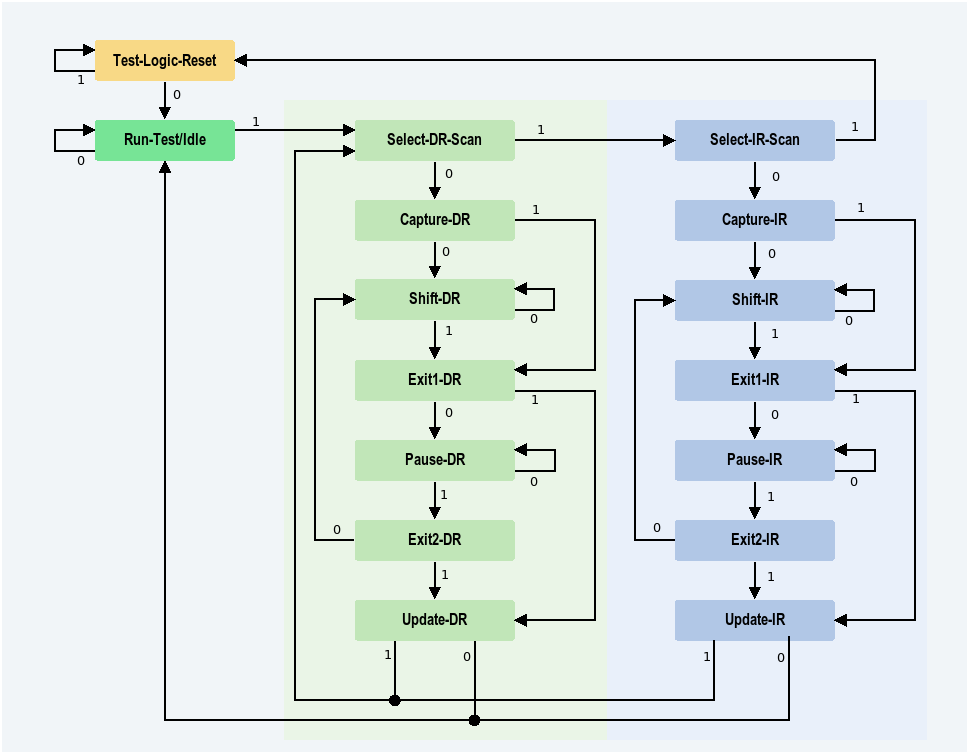
\includegraphics[width=0.75\columnwidth]{state.png}
        \caption{TAP state machine introduced in the IEEE 1149.1}
        \label{fig:state}
    \end{figure}
\end{frame}

% TODO needs more accurate info
\begin{frame}
    \frametitle{An Example of TAP Controller Opcodes}
    \note[item]{BYPASS, EXTEST, SAMPLE, and PRELOAD are rquired by standard}
    \note[item]{for EXTEST: Signals from the outside of the component are loaded at the falling edge of TCK in Capture-DR state.
    Signals from the inside of the component are loaded on the falling edge of the TCK in Update-DR state.}
    \note[item]{EXTEST: output is defined by BSC at Update-DR, signal recieved will be put into BSC on Capture-DR}
        \begin{tabular}{|c|p{8cm}|}
            \hline
            Opcode & Description \\
            \hline
            BYPASS & Connects TDI and TDO for faster access between chains. \\
            \hline
            SAMPLE & Take a snapshot from the state of the components boundary scan register. \\
            \hline
            PRELOAD & Load the date into the boundary scan register. \\
            \hline
            EXTEST & Select the boundary scan register as input and output of the selected chip. \\
            \hline
            IDCODE & Select the device identification register. \\
            \hline
            DPACC/APACC & Access the arm specific access port and debug port registers.\\
            \hline
        \end{tabular}
\end{frame}

\subsection{Debugging in ARM}
\begin{frame}
    \frametitle{Serial Wire Debug: A JTAG alternative?}
    \note[item]{This interface was defined in ARM Debug
    Interface v5 Architecture Specification.}
    \note[item]{Uses 2-pins vs 5-pins of jtag.}
    \note[item]{Removes the daisy-chain architecture, in which the speed is limited by the slowest link.}
    \note[item]{But it is limited to the arm architecture.}
    \note[item]{Jtag targets are limited to 10Mhz sometimes they go up to 100Mhz}
    SWD:
    \begin{itemize}
        \item 2-pin input.
        \item Backward compatible.
        \item Up to 4 MB/s at 50 MHz.
        \item No bottleneck in chains.
    \end{itemize}
\end{frame}

\begin{frame}
    \frametitle{JTAG as a Debugger!?}
    \note[item]{All ARMv7 and ARMv9 Cores have halt mode debugging.}
    \note[item]{ARM core macrocell is deeply embedded. So to modify signals we
    have a TAP controller with boundary scan register around core signals.}
    \note[item]{using these scan chains we can set break points and observe
    data and instructions and change them.}
    \note[item]{scan chain one is the core signals}
    \note[item]{On ARMv9 Devices there is a scan chains that corresponds to the
    Instruction Bus and the Data Bus.}
    Embedded-ICE usage:
    \note[item]{Hardware breakpoint is a comparator, there are variation such
    as specific instruction or on an specific instruction address.}
    \note[item]{Software breakpoint replace a instruction in address space
    with a special instruction to force it into debug state.}
    \note[item]{The debugger must ensure cache coherency after changing the
    state: disable line fills, examine cache for write policy, and
    invalidate instruction cache}
    \begin{itemize}
        \item Debug Request: Sets the core in the debugger.
        \item Hardware Breakpoints.
        \item Software Breakpoints.
        \item Watchpoints: Hardware breakpoints on data bus.
        \item Vector Catching: Catch the interrupt vectors and exceptions.
        \item Single Stepping: Renter the debug state after one instruction.
    \end{itemize}
\end{frame}

\begin{frame}
    \frametitle{OpenOCD}
    Opensource debugger:
    \note[item]{Tool Command Language, Tickle.}
    \begin{itemize}
        \item GDB interconnection.
        \item Single stepping.
        \item Breakpoints.
        \item Watchpoints.
        \item Embedded Tcl interpreter.
        \item Embedded flash driver.
    \end{itemize}
\end{frame}

\subsection{JTAG Controllers}
\begin{frame}[t]
    \frametitle{JTAG Controllers}
    There are many JTAG controllers available for use:
    \note[item]{Software support and TPIU}
    \begin{itemize}
        \item 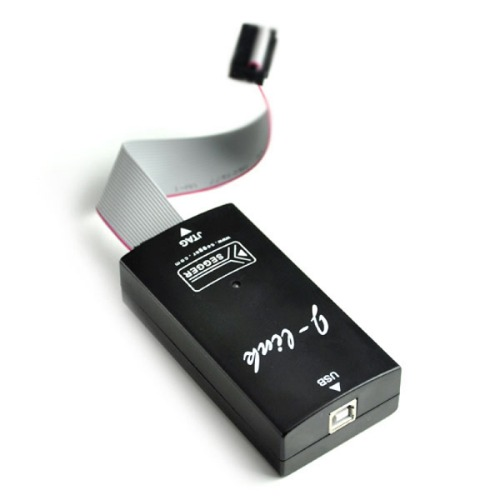
\includegraphics[width=2.8cm,valign=c]{jlink.jpg} J-Link, 398\$
        \item 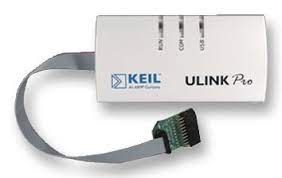
\includegraphics[width=2.8cm,valign=c]{ulink.jpeg} Keil U-Link Pro, 695\$
        \item 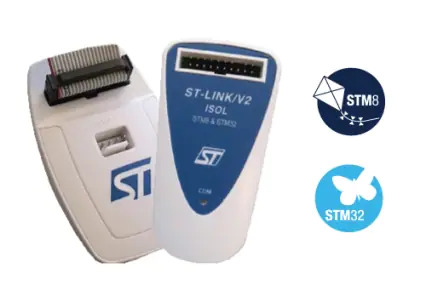
\includegraphics[width=2.8cm,valign=c]{stlink.jpg} ST-Link v3, 35\$
    \end{itemize}
\end{frame}

\section{ARM CoreSight}
\begin{frame}
    \frametitle{ARM CoreSight}
    \note[item]{ECT: Pass the debug events from one core to another.}
    \note[item]{CTI: The CTI combines and maps the trigger requests,
    and broadcasts them to all other interfaces on the ECT as channel events.}
    \note[item]{CTM: This block controls the distribution of channel events.
    It provides Channel Interfaces (CIs) for connection to either CTIs or CTMs.
    This enables multiple CTIs to be linked together.}
    \note[item]{Links provide connection, triggering, and flow of traced data.
    For example ARM Trace Funnel combines several trace sources onto a single
    ATB bus (AMBA Trace Bus) or AMBA 2.}
    \note[item]{Advanced eXtensible Interface or AMBA 3}
    \note[item]{Advanced Microcontroller Bus Architecture, AMBA high performance Bus, AHB}
    \note[item]{Trace sink: Trace Port Interface Unit.}
    \note[item]{ETB rangers from 4KB to 64KB}
    \note[item]{TPIU: Trace Port Interface Unit 800Mb/s Keil Ulink Pro}
    ARM CoreSight, Debugging and Tracing Solution:
    \begin{itemize}
        \item Control interfaces.
        \item Trace sources.
        \item Trace links.
        \item Trace sinks.
        \item Debug and access ports.
    \end{itemize}
\end{frame}

\subsection{Trace Sources}
\begin{frame}
    \frametitle{Trace Sources}
    ARM CoreSight Trace Sources:
    \begin{itemize}
        \item Embedded Trace Macrocell (ETM).
        \item Program Trace Macrocell (PTM).
        \item Instrumentation Trace Macrocell (ITM).
        \item System Trace Macrocell (STM).
        \item AMBA Trace Macrocell (HTM).
    \end{itemize}
\end{frame}
\begin{frame}
    \frametitle{Embedded Trace Macrocell}
    \note[item]{particular etm might not support data trace}
    \note[item]{This macrocell permits instruction and data trace. ETM data is compressed
    and encoded and therefore should be decompressed and decoded before use. \\
    Triggers and filters control ETM trace data generation. Filters allow to
    control how much data is produced. This is useful if:}
    \note[item]{enable on ICE events}
    Features:
    \begin{itemize}
        \item Instruction trace.
        \item Data trace.
        \item Triggers.
        \item Filters.
    \end{itemize}
\end{frame}

\begin{frame}
    \frametitle{ETM Filters}
    \note[item]{ARM CoreSight ETM-XXX Techincal Reference Manual }
    \begin{itemize}
        \item Exception Level.
        \item Conditional code mode tracing.
        \item Comparators:
            \begin{itemize}
                \item Data.
                \item Address.
            \end{itemize}
        \item External pin inputs.
    \end{itemize}
\end{frame}

\begin{frame}
    \frametitle{ETM Output}
    \begin{itemize}
        \item Event timestamping.
        \item Cycle accurate tracing.
        \item Conditional instruction status.
        \item Atomic instruction status.
        \item Hypervisor mode.
        \item Data accesses from cores.
    \end{itemize}
\end{frame}

\begin{frame}
    \frametitle{Program Trace Macrocell}
    \note[item]{Program Trace Macrocell (PTM) is only found in systems before Armv8.
    PTMs perform instruction trace only. It is works the same as the ETM does.}
    \begin{itemize}
        \item Found in systems before ARMv8.
        \item Instruction trace only.
        \item Predecessor to ETM.
    \end{itemize}
    Might not overlap with ETM on old core architectures.
\end{frame}

\begin{frame}
    \frametitle{Instrumentation Trace Macrocell}
    \note[item]{The Instrumentation Trace Macrocell (ITM) is a low-bandwidth,
    application-driven trace source. The ITM is mainly used to:}
    Features:
    \begin{itemize}
        \item Support \textit{printf}-style debugging.
        \item Trace OS and application events.
        \item Output diagnostic system information.
        \item Able to log time critical code.
    \end{itemize}
    \note[item]{Why use ITM: using printf and logging distrubs time critical
    applications and is unacceptable.}
    \note[item]{performance potential and overhead??}
\end{frame}

\begin{frame}
    \frametitle{System Trace Macrocell}
    Features:
    \begin{itemize}
        \item Successor to ITM.
        \item A dedicated Advance eXtensible Interface for recieving trace
            information
        \item Multiple processors and cores can share one system trace
            macrocell
        \item Ability to have a larger buffer.
    \end{itemize}
\end{frame}

\begin{frame}
    \frametitle{AMBA Trace Macrocell}
    \note[item]{The HTM is a real-time trace module capable of address and data tracing
    of the AHB bus. This macrocell is able to generate events that can be
    used by other macrocells inside the system.}
    Features:
    \begin{itemize}
        \item data and address tracing.
        \item Dummy bus slave to create traffic.
        \item Make IO and memory accesses visible.
        \item Correlate trace output with other trace macrocells.
    \end{itemize}
\end{frame}

\subsection{OpenCSD}
\begin{frame}
    \frametitle{OpenCSD}
    \note[item]{OpenCSD is built by linaro to parse the ARM CoreSight output data.
    This library has extensible support for ARM CoreSight components but is
    lacking in some areas:}
    \note[item]{Linaro works on software that is close to the silicon such as
    kernel, multimedia, power management, graphics and security.}
    \note[item]{the team works directly with upstream projects supporting core
    technologies including Linux kernel core features, power management,
    security, toolchain support (both GCC and LLVM), testing and CI and
    Virtualization}
    Linaro:
    \begin{itemize}
        \item Opensource company.
        \item Working on software that is close to silicon.
        \item Co-maintaining support projects
    \end{itemize}
    Features:
    \begin{itemize}
        \item Deformat.
        \item Process.
        \item Decode.
    \end{itemize}
    \note[item]{Frame Deformatting : Removal CoreSight frame formatting from individual trace streams.}
    \note[item]{Packet Processing : Separate individual trace streams into discrete packets.}
    \note[item]{Packet Decode : Convert the packets into fully decoded trace describing the program flow on a core.}
    Lacking in:
    \begin{itemize}
        \item ITM software tracing support.
        \item ETMv3 data trace, packet decoding.
        \item ETMv4 data trace, packet processing and decoding.
    \end{itemize}
\end{frame}

\subsection{Sample Output}
\begin{frame}
    \frametitle{Sample Output Of the Embedded Trace Macrocell}
    \begin{figure}
        \centering
        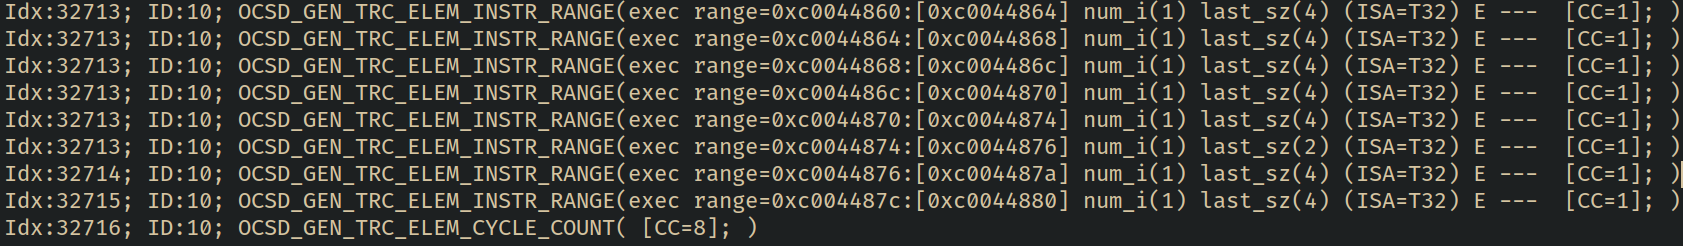
\includegraphics[width=1.0\columnwidth]{out.png}
        \caption{An Example Output of ETM}
        \label{fig:out}
    \end{figure}
\end{frame}

\begin{frame}
    \frametitle{Where to Go Next?!}
    \begin{itemize}
        \item More digging on cycle accuracy.
        \item Measure the overhead of STM or ITM.
        \item Correlate The HTM and ETM output.
    \end{itemize}
\end{frame}

\begin{frame}
    \frametitle{References}
    \begin{itemize}
        \item IEEE Std 1149.1-2001, IEEE Standard Test Access Port and Boundary-Scan Architecture
        \item University of Applied Sciences Augsburg ,Department of Computer Science, Open On-Chip Debugger, Dominic Rath
        \item Arm CoreSight Architecture Specification v3.0, ARM
        \item Understanding Trace, Trace Overview, ARM
        \item Embedded Trace Macrocell Architecture Specification, ARM
        \item Learn The Architecture, ARM
        \item ARM Debug Interface v5 Architecture Specification, ARM
    \end{itemize}
\end{frame}

\begin{frame}
  \centering \Large
  \emph{Thank You For Your Attention}
\end{frame}

\end{document}
